\documentclass[uplatex,dvipdfmx,a4j,12pt]{jsarticle}

\usepackage[utf8]{inputenc}
\usepackage{graphicx}
\usepackage{amsmath}
\usepackage{comment}
\usepackage{color}
\usepackage{url}
\usepackage{siunitx}
\usepackage[version=4]{mhchem}
\usepackage{paralist}
\usepackage{longtable}
\usepackage{multirow}
\usepackage[dvipdfmx]{hyperref}
\usepackage{pxjahyper}
\usepackage{here}
\usepackage{subcaption}
\usepackage{enumitem}
\usepackage{float}
\setlist[description]{parsep=5pt}
\setlist[enumerate]{parsep=5pt}

% 半角文字のパーセント、より右側は、コメントとして扱われます。

% タイトルページの内容をここで記述します。
\title{
  物理学実験IIレポート\\    % \\ は、強制的に改行するコマンドです。
  課題9 「素粒子の相互作用と磁気モーメント」
  }
\author{
  実験回: 第x回 \\
  氏名: \\
  実験者番号:
  \\
  共同実験者:
  }
\date{
  実験日:2025年 x月 x日~ x月 x日 \\
  提出日:2025年 x月 x日}  % 実験日と、提出日を記入して下さい

% ここから本文が始まります。
\begin{document}

% 上で設定したタイトルページの情報は、\maketitle があって始めて、コンパイル後に表示されます。
\maketitle

% レポートのフィードバックのコメントを希望しない場合には、
% 48行目から55行目までをコメントアウト(行頭に%を入れる)。
% コメントを希望する場合は、何について聞きたいかを具体的に書いて下さい。

% 縦方向の空白を挿入するコマンドです。em は行の高さ分、を意味する単位です。
\vspace{2em}
\begin{center}
    \begin{minipage}{0.5\linewidth}
        レポートのコメントを希望します。

        具体的には、○○について評価を下さい。
    \end{minipage}
\end{center}

\vspace{5em}  


% 概要は論文・レポート全体を一つの段落にまとめたものです。
% 物理の分野では、概要では段落分けをしません。
%
\begin{abstract}
    \textcolor{red}{このテンプレートにある指示文章は全て削除し、自分で書いた文章に差し替えること。残っていた場合は読みやすさを損ねるため減点とする。}
    (概要ではレポートの概要を簡潔に記述せよ。例えば、以下のようなものである。)
    ○○の目的のために、■■の実験を行った。
    その結果△△であることが確かめられた。
\end{abstract}

% 強制的に改ページを行う
\newpage


\section{目的}
この実験のねらいが何であるかを、テキストを参考に簡潔にまとめる。


\section{原理}
\subsection{素粒子の相互作用}
最も基本的な粒子である素粒子は,そのスピンや電荷などの性質によって大別される.
図\ref{fig:particle}に素粒子の分類を示す.

\begin{table}[H]
  \centering
  \caption{素粒子の分類}
  \label{fig:particle}
  \begin{minipage}{\linewidth}
    \centering
    \begin{tabular}{cccccc}
      \hline
      & スピン & 電荷 & 第1世代 & 第2世代 & 第3世代 \\
      \hline\hline
      \multirow{2}{*}{クォーク} & \multirow{2}{*}{$\frac{1}{2}$} & $+\frac{2}{3}$ & $u$ & $c$ & $t$ \\
      & & $-\frac{1}{3}$ & $d$ & $s$ & $b$ \\
      \hline\\
    \end{tabular} 
  \end{minipage}

  \begin{minipage}{\linewidth}
    \centering
    \begin{tabular}{cccccc}
      \hline
      & スピン & 電荷 & 電磁相互作用 & 弱い相互作用 & 強い相互作用 \\
      \hline\hline
      \multirow{2}{*}{レプトン}  & \multirow{2}{*}{$\frac{1}{2}$} & 0 & $\nu_e$ & $\nu_\mu$ & $\nu_\tau$ \\
      & & $-1$ & $e^{-}$ & $\mu^{-}$ & $\tau^{-}$ \\
      \hline
      \multirow{2}{*}{ゲージ粒子} & \multirow{2}{*}{1} & 0 & $\gamma$ & $Z^0$ & $g$\\
      & & $\pm1$ & -- & $W^{\pm}$ & -- \\
      \hline\\
    \end{tabular}
  \end{minipage}

  \begin{minipage}{\linewidth}
    \centering
    \begin{tabular}{ccc}
      \hline
      & スピン & 電荷  \\ 
      \hline\hline
      ヒッグス粒子 & 0 \\
      \hline
    \end{tabular}
  \end{minipage}
\end{table}

ここで,クォークやレプトンは物質を構成する粒子であり,それぞれが第1世代から第3世代まで存在する.
また,ゲージ粒子やヒッグス粒子は,素粒子間の相互作用を媒介する粒子である.
この相互作用は,電磁相互作用,弱い相互作用,強い相互作用,および重力相互作用の4種類に分類される.

電磁相互作用は、電荷を持つ粒子間で働く相互作用であり、光子($\gamma$)が媒介する。
一方で,弱い相互作用,強い相互作用はそれぞれ弱荷を持つクォークとレプトン,カラー荷を持つクォーク間で働く相互作用であり,
電磁相互作用に対する力との相対的な強さから,その名が付けられている.
また,重力相互作用は質量を持つ粒子間で働く相互作用であるが,他の相互作用と比較して非常に弱いため,素粒子実験においては無視されることが多い.
一方で,唯一斥力をもたない重力相互作用は.力が相殺されることがなく遠くまで伝わるため,宇宙規模の現象を説明する上で重要な役割を果たす.

\subsection{磁気モーメント}
円電流が作る磁場を考えると,磁気 (双極子) モーメント$\boldsymbol{\mu}$を用いて次のように表される.
\begin{gather}
  \mathbf{A}(\mathbf{r}) = \frac{\mu_0}{4\pi}\frac{\boldsymbol{\mu}\times\hat{\mathbf{r}}}{r^2},\\
  \mathrm{B} = \nabla \times \mathbf{A}(\mathbf{r}) = \frac{\mu_0}{4\pi}\frac{3(\boldsymbol{\mu}\cdot\hat{\mathbf{r}})\hat{\mathbf{r}}-\boldsymbol{\mu}}{r^3},
\end{gather}
ここで,磁気双極子モーメントは円電流$I$と円電流が囲む面積$S_a \mathbf{n}$ ($\mathrm{n}$は面の法線方向) を用いて,
\begin{gather}
  \boldsymbol{\mu} = IS_a \mathbf{n},
\end{gather}
と定義される.

以上の議論をもとに,電荷$+e$, 質量$m$を持ち,等速円運動する粒子について考えると,その角運動量は,
\begin{gather}
  \mathbf{L} = \mathbf{r}\times\mathbf{p} = m \mathbf{r}\times\mathbf{v} = mvr \mathbf{n} 
\end{gather}
で表される.
一方で,磁気双極子モーメントは,
\begin{gather}
  \boldsymbol{\mu} = IS_a \mathbf{n} = \frac{ev}{2\pi r} \pi r^2 \mathbf{n}
\end{gather}
つまり,磁気双極子モーメントと各運動量の間の関係として,
\begin{gather}
  \boldsymbol{\mu} = \frac{e}{2m}\mathbf{L},
\end{gather}
が導かれる.

素粒子の場合はさらに軌道角運動量$\mathbf{L}$に加えて,素粒子固有の内部自由度に起因するスピン角運動量$\mathbf{S}$が存在する.
このとき,スピン角運動量も含めた磁気双極子モーメントは,
\begin{gather}
  \boldsymbol{\mu} = \frac{e}{2m}(\mathbf{L} + g\mathbf{S}),
\end{gather}
と表される.
ここで,$g$はLand\'e の $g$因子と呼ばれる定数である.






\subsection{ミューオンに働く相互作用}

% 教科書の$\S1\sim\S3$を参考に、実験に関連する原理を記述する。特に、
% \begin{itemize}
%     \item 素粒子の相互作用
%     \item 磁気モーメント
%     \item ミューオンに働く相互作用
% \end{itemize}
% についての説明は必ず記述すること。

\section{実験装置}
% 実験装置について、その構成について説明し、特に何を何の目的でどのように配置しているのかに留意して説明する。

\section{課題1: ミューオン崩壊事象の測定}
\subsection{方法}
まず始めに,シンチレーションカウンタの動作確認を行った.
ここでは,光電子増倍管 (PMT) に適当な電圧を印加した際にシンチレータから信号が得られるのを確認した.
PMTには熱雑音などからくる信号も計測されるが,同じプレートに接続された2つのPMTからの同時信号のみを計測することでこの雑音を除去することができる.
そこで,電圧を上げて同時計数を確認し,適当な電圧で計数が一定になるまたは一般に期待される80 count/sec程度になることを確認した.
この過程を上段,中段,下段 (それぞれPlate 1, Plate 2, Plate 3) の各シンチレータで確認し,以降の実験ではそれぞれこの電圧で測定を行った.

次に.ミューオンフラックスの測定実験を行った.
ここでは,上段と中段シンチレータの信号を用い,コインシデンス回路を用いて同時計測を行うことで,ミューオンフラックスの計数を行った.
上から降り注ぐ宇宙線の大半はミューオンであるため,同時計測によって他の影響を排してミューオンフラックスを測定することができる.

以上の確認の後に,3枚のシンチレータから出力される信号のタイミングから,ミューオン崩壊事象の測定を行った.
計数ブロック図を図\ref{fig:block}に示す.
\begin{figure}[H]
  \centering
  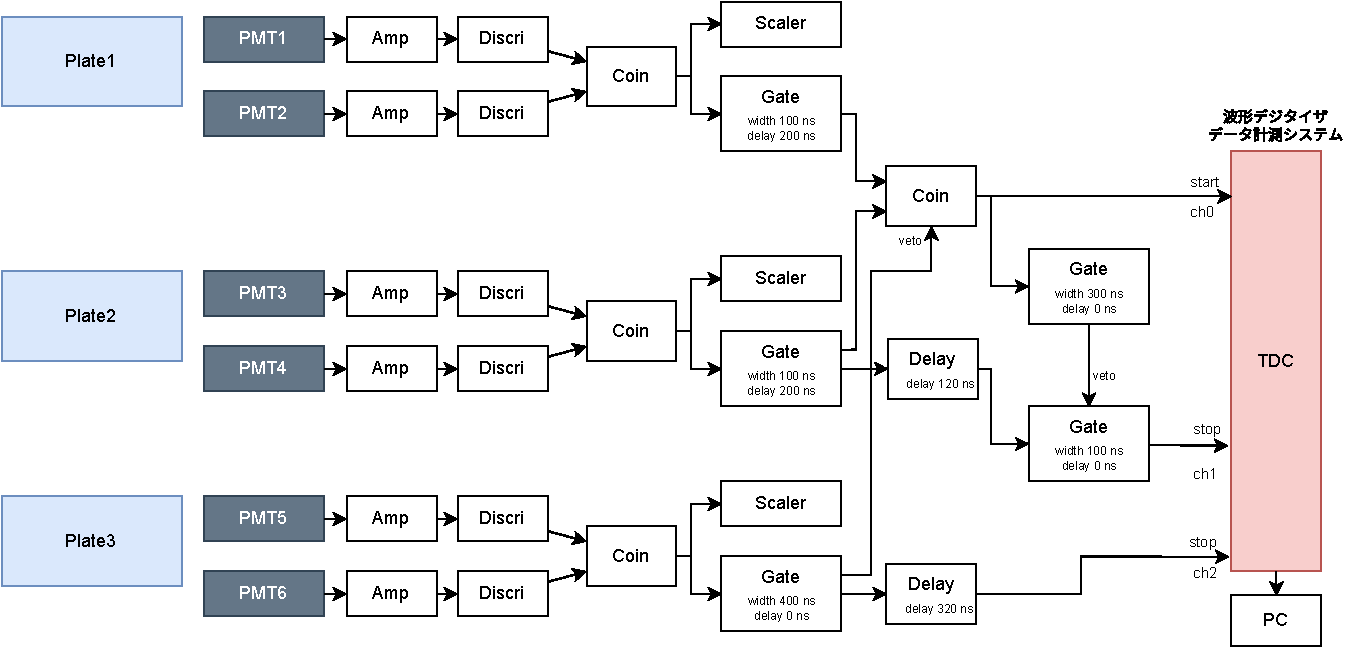
\includegraphics[width=0.95\linewidth]{img/block.pdf}
  \caption{ミューオン崩壊事象の計数ブロック図}
  \label{fig:block}
\end{figure}
飛来したミューオンが銅板で静止する場合,上段および中段のシンチレータでほぼ同時に計測された後,
銅板で止められ崩壊して放出される電子または陽電子が中段または下段のプレートを通過して計測される.
このとき,銅板で静止しない場合や銅板のない領域を通過する場合,下段のシンチレータは上中段のシンチレータとほぼ同時に信号を出力するため,
これを利用して崩壊事象でない事象を除外することができる.

また,計測を開始する前に,計測器 (TDC) のキャリブレーションを行った.
TDCでは時間差をデジタル数値 (TDC Channel) で計測するため,時間差とTDC Channelの関係を調べる必要がある.
さらに,このキャリブレーションに加え,実際には回路等から生じる時間差があるために,同時に起こる事象に対しても測定される時間差にはオフセットが存在する.
そこで,図\ref{fig:block}中のveto信号を一度無くして1分間計測を行った.
このときに観測される事象はその殆どが銅板でミューオンが静止せずに通り抜ける事象であり,
これはほぼ同時に発生するため,この計測からオフセットを求めることができる.

以上のキャリブレーションとオフセット測定の後に約6日間計測を行い,ミューオン崩壊事象の計数を行った.

\subsection{結果}
まず始めに,PMTから信号波形を図\ref{fig:waveform}に示す.
% \begin{figure}[H]
%   \centering
%   \includegraphics[width=0.85\linewidth]{analysis/waveform.pdf}
%   \caption{PMTからの信号波形.}
%   \label{fig:waveform}
% \end{figure}

次に,上中下段のシンチレータについて印加する電圧と得られた信号数の関係を図\ref{fig:cout-vs-voltage}に示す.
また,特に図\ref{fig:coincidence}に印加する電圧と同時計数率の関係を示す.
測定の結果,上段では1700 V, 中段では1750 Vにおいて同時計数率が80 count/sec 程度となったため,
以降はこの電圧値において計測を行った.
一方で,下段では1750 Vにおいても同時計数率が45 count/sec 程度であったが,印加できる電圧の上限が1750 Vであったため,以降この電圧で計測を行った.

\begin{figure}[H]
  \centering
  \begin{minipage}{0.85\linewidth}
    \centering
    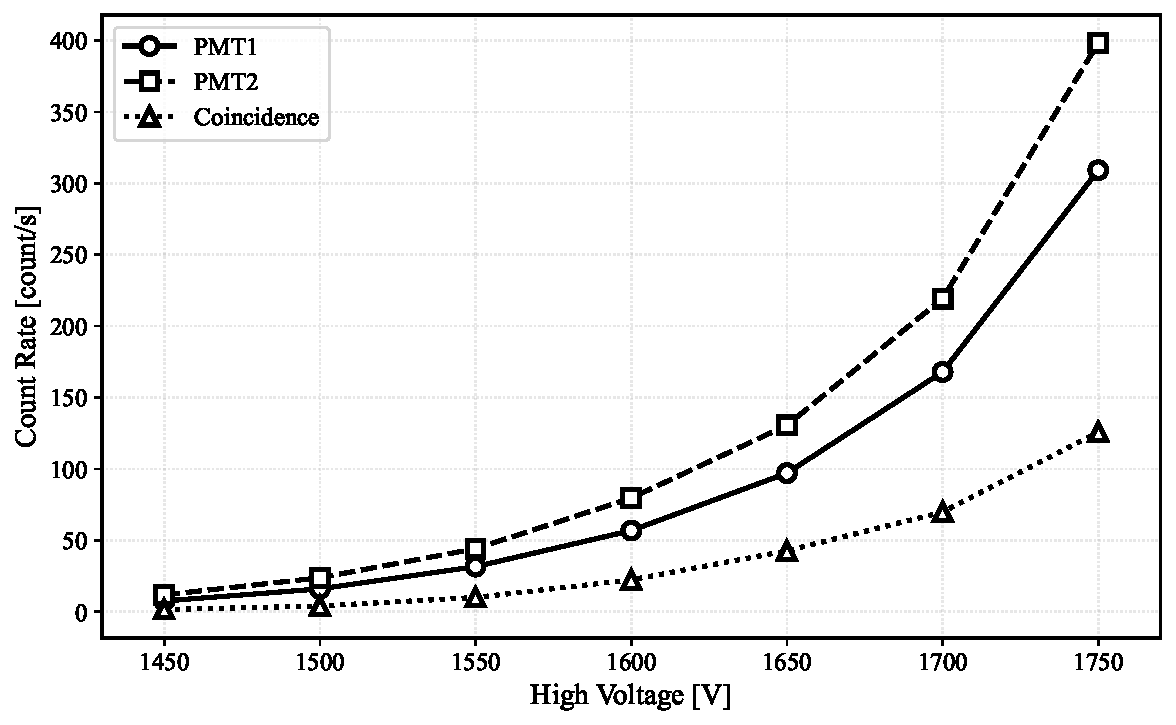
\includegraphics[width=\linewidth]{analysis/plate1_count_vs_voltage.pdf}
    \subcaption{上段シンチレータの電圧と計数.}
    \label{fig:upper}
  \end{minipage}
  
  \begin{minipage}{0.85\linewidth}
    \centering
    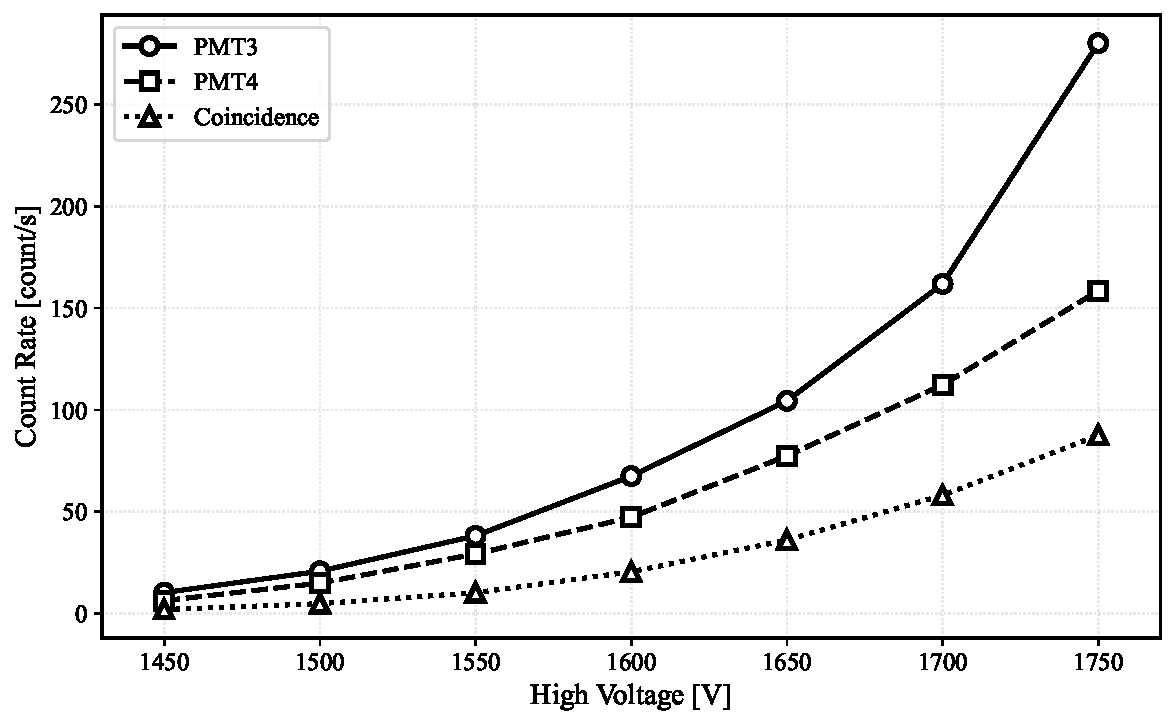
\includegraphics[width=\linewidth]{analysis/plate2_count_vs_voltage.pdf}
    \subcaption{中段シンチレータの電圧と計数.}
    \label{fig:middle}
  \end{minipage}
\end{figure}

\begin{figure}[H]
  \ContinuedFloat
  \centering
  \begin{minipage}{0.85\linewidth}
    \centering
    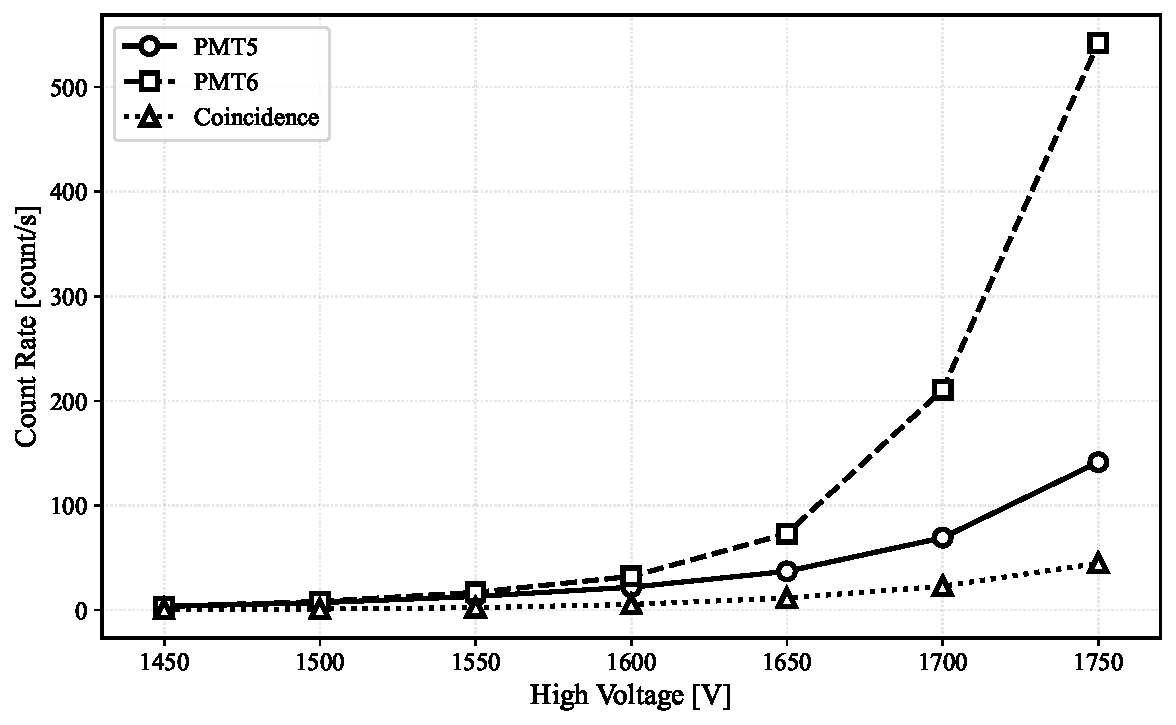
\includegraphics[width=\linewidth]{analysis/plate3_count_vs_voltage.pdf}
    \subcaption{下段シンチレータの電圧と計数.}
    \label{fig:lower}
  \end{minipage}
  \caption{シンチレータの電圧と計数.}
  \label{fig:cout-vs-voltage}
\end{figure}

\begin{figure}[H]
  \centering
  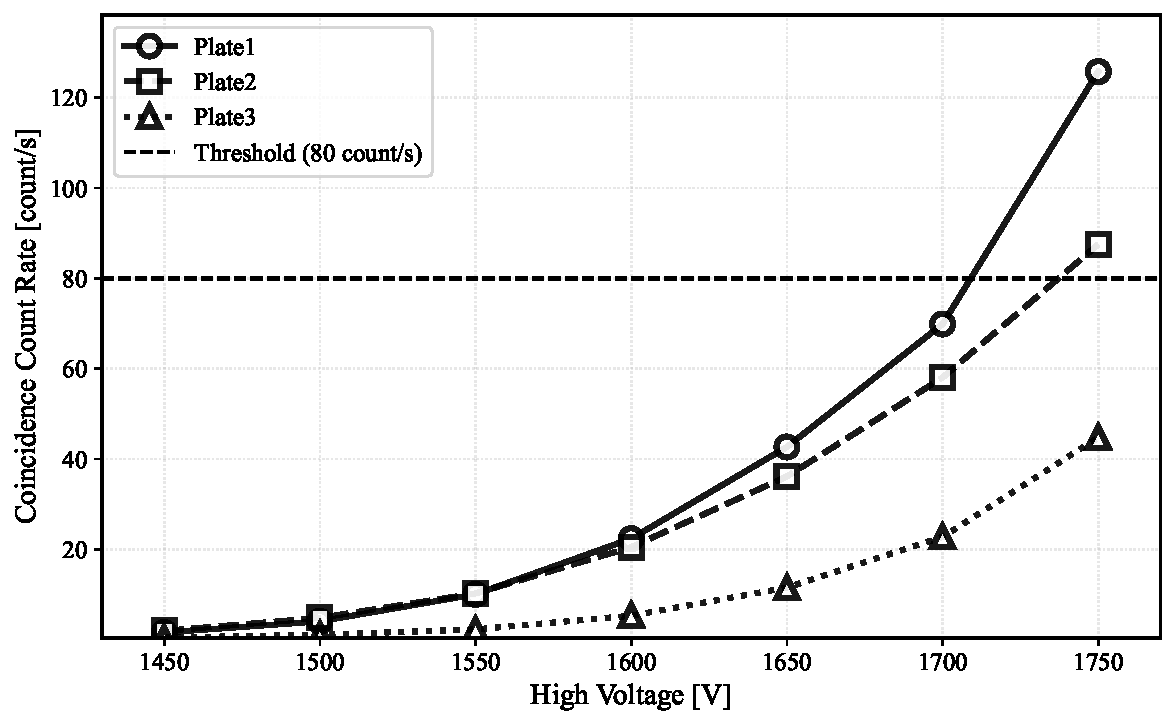
\includegraphics[width=0.85\linewidth]{analysis/comparison_coincidence_rates.pdf}
  \caption{上中段シンチレータの同時計数率.}  
  \label{fig:coincidence}
\end{figure}

\enskip

次に,ミューオンフラックスの測定実験の結果を述べる.

1分間の同時測定の結果,上段・中段の同時計数率は$n = 6.2$ [count/s] であった.
上段,中段のプレート面積はそれぞれ $S_1 = 0.50 \,[\mathrm{m}^2]$, $S_2 = 0.74 \,[\mathrm{m}^2]$, プレート間距離は$L = 0.88 \,\mathrm{[m]}$であった.
したがって,中段プレートのある点から上段プレートを見込む立体角$\Omega$は, $L \gg S_1$の条件のもとで次のように近似できる :
\begin{gather}
  \Omega = \frac{S_1}{L^2} = \frac{0.50 \,[\mathrm{m}^2]}{(0.88 \,[\mathrm{m}])^2} \approx 0.65 \, [\mathrm{sr}],
\end{gather}
となる.
これを中段のプレート面積で積分することでアクセプタンス$A$を求めると,
\begin{gather}
  A = \Omega S_2 = 0.65 \, [\mathrm{sr}] \times 0.74 \, [\mathrm{m}^2] \approx 0.48 \, [\mathrm{m}^2 \cdot \mathrm{sr}],
\end{gather}
したがって,同時計数率をアクセプタンスで規格化してミューオンフラックスを求めると,
\begin{gather}
  \Phi = \frac{n}{A} = \frac{6.2 \, [\mathrm{count/s}]}{0.48 \, [\mathrm{m}^2 \cdot \mathrm{sr}]} \approx 12.9 \, [\mathrm{/(s\cdot m^2\cdot sr)}],
\end{gather}

\enskip

最後に,ミューオン崩壊事象の測定結果について述べる.

まず始めに,TDCのキャリブレーション結果を図\ref{fig:calibration}に示す.
横軸がTDCで計測されたデジタル数値 (TDC Channel) であり,縦軸が回路を作成して設計された時間差 (ns) である.
\begin{figure}[H]
  \centering
  \begin{minipage}
    {0.85\linewidth}
    \centering
  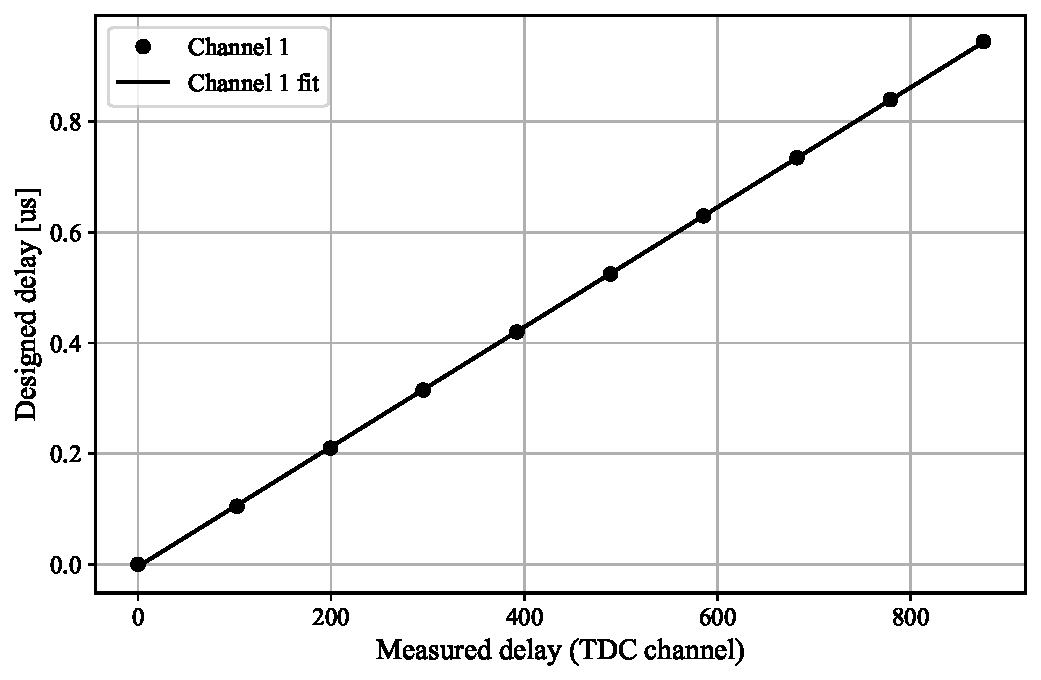
\includegraphics[width=0.85\linewidth]{analysis/calibration_channel_1.pdf}
    \subcaption{Ch.1のキャリブレーション測定.}
    \label{fig:calib1}
  \end{minipage}
  \begin{minipage}
    {0.85\linewidth}
    \centering
  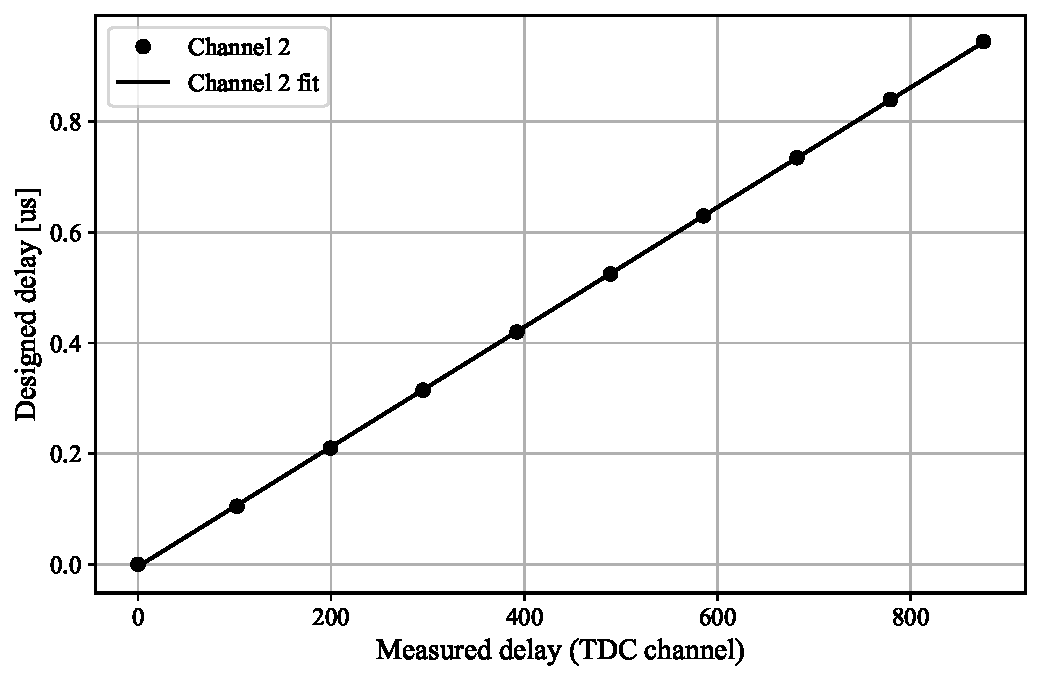
\includegraphics[width=0.85\linewidth]{analysis/calibration_channel_2.pdf}
    \subcaption{Ch.2のキャリブレーション測定.}
    \label{fig:calib2}
  \end{minipage}  
  \caption{TDCのキャリブレーション測定.}
  \label{fig:calibration}
\end{figure}

また最小二乗法によるフィッティングの結果は,それぞれ以下のようになった.
\begin{align}
\begin{cases}
\,\mathrm{Ch.1} : Y = 0.00108 X - 0.00409, \quad R^2 = 1.00,\\   
\,\mathrm{Ch.2} : Y = 0.00108 X - 0.00416, \quad R^2 = 1.00.
\end{cases}
\end{align}

また,回路によって生じる時間差を計測した結果を表\ref{tab:offset}に示す.
\begin{table}[H]
  \centering
  \caption{回路による時間差の測定結果.}
  \label{tab:offset}
  \begin{tabular}{ccc}
    \hline
    TDC Channel & 時間差 [TDC Channel] & オフセット [\si{\micro\second}] \\
    \hline
    Ch.1 & -1.00 & -0.00518 \\
    Ch.2 & 45.0 & 0.0446 \\
    \hline
  \end{tabular}
\end{table}

以上の測定結果をもとに,同時信号とその時間差からミューオン崩壊事象の計数を行った結果を図\ref{fig:muon_decay}に示す.
ここで,崩壊時間が短いデータ ($\Delta t < 10$\, [\si{\micro\second}]) および長いデータ ($\Delta t > 10$\, [\si{\micro\second}]) は除外している.
これは,極端に崩壊時間が短いデータや長いデータには熱雑音など他の影響による事象が含まれる可能性が高いと考えられるためである.

また,図\ref{fig:muon_decay}には,崩壊曲線として指数関数型の$Y = A e^{-X/\tau} + C$をフィッティングした結果も示している.
ここで$\tau$がミューオンの寿命であり,定数項$C$は背景雑音の影響を取り入れるために導入している.

\begin{figure}[H]
  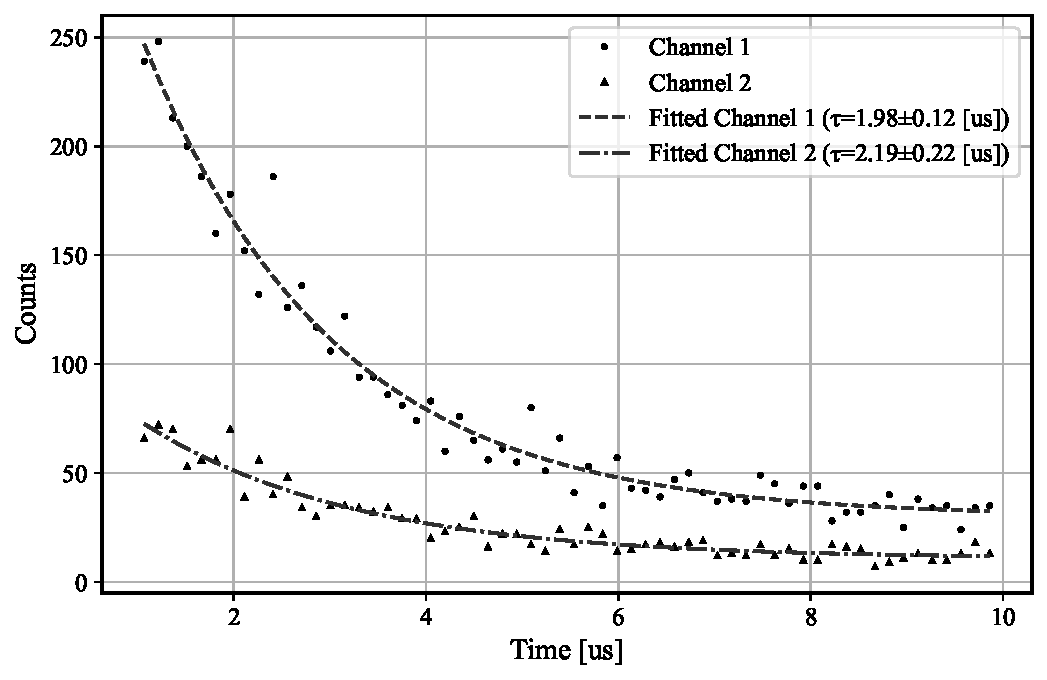
\includegraphics[width=0.85\linewidth]{analysis/lifetime_measurement.pdf}
  \caption{ミューオン崩壊事象の計数.}
  \label{fig:muon_decay}
\end{figure}






\subsection{考察}

\section{課題2: 一様磁場の生成}
\subsection{方法}

\subsection{結果}

\subsection{考察}


\section{課題3: ミューオン磁気モーメントの測定}
\subsection{方法}

\subsection{結果}

\subsection{考察}

\section{設問への解答}


\section{結論}

実験目的を要約して記述し、それに対応する結論を最後に記述すること。

% 参考文献は、各課題に合わせて必要なものに書き換えること
\begin{thebibliography}{9}

    \bibitem{bunken1}
        A. Einstein, B. Podolsky, and N. Rosen, 
        Phys. Rev. \textbf{47}, (1935) 777.
        % いわゆるEPRパラドックスと呼ばれる量子力学に関する論文

    \bibitem{bunnken2}
        J.J. Aubert \textit{et al.},
        Phys. Lett. B \textbf{123} (1983) 275.
        % いわゆるEMC効果と呼ばれる現象についての実験の論文
    
\end{thebibliography}

\end{document}
